% Source: AESP_466_ClassWork/Supplements/Companion/Euler_Sequences_Quaternions/Euler_Sequences_Quaternions.tex

\documentclass[border=4pt]{standalone}
\usepackage{amsmath}
\usepackage{amssymb}
\usepackage{graphicx}
\usepackage{tikz}
\usepackage{xcolor}
\usetikzlibrary{shapes.geometric, arrows.meta, positioning, decorations.pathmorphing, decorations.pathreplacing, patterns, calc, 3d}

\definecolor{Garnet}{HTML}{73000A}
\definecolor{USC_Rose}{HTML}{CC2E40}
\definecolor{USC_Blue}{HTML}{466A9F}
\definecolor{USC_Slate}{HTML}{1F414D}
\definecolor{USC_Olive}{HTML}{65780B}
\definecolor{USC_Lime}{HTML}{CED318}
\definecolor{USC_Gold}{HTML}{A49137}
\definecolor{USC_Black90}{HTML}{565656}
\definecolor{USC_Black10}{HTML}{ECECEC}

\newcommand{\sectionheader}[1]{%
  \vspace{0.5cm}
  {\noindent\Large \textbf{#1}}
  \vspace{0.2cm}
  \hrule
  \vspace{0.1cm}
  \hrule
  \vspace{0.3cm}
}

\begin{document}
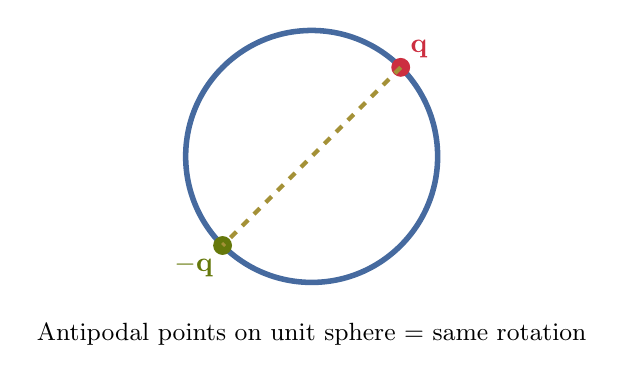
\begin{tikzpicture}[scale=0.8]
    \draw[line width=2pt, USC_Blue] (0,0) circle (2);
    \filldraw[USC_Rose] (1.414, 1.414) circle (4pt) node[above right] {$\mathbf{q}$};
    \filldraw[USC_Olive] (-1.414, -1.414) circle (4pt) node[below left] {$-\mathbf{q}$};
    \draw[dashed, USC_Gold, line width=1.5pt] (1.414, 1.414) -- (-1.414, -1.414);
    \node[below, font=\small] at (0,-2.5) {Antipodal points on unit sphere = same rotation};
\end{tikzpicture}
\end{document}
